\chapter{Структурный и системный анализ исследуемого объекта}

Рассмотрим популярные платформы, которые предоставляют функционал по созданию 
информационных аватаров для общения. В последние годы интерес к цифровым двойникам и 
аватарам значительно вырос, что привело к появлению множества сервисов, предлагающих 
пользователям возможность создавать виртуальные образы реальных или вымышленных личностей. 
Несмотря на разнообразие решений, концептуально платформы во многом близки по духу, 
предоставляя пользователям функционал, основанный на конфигурационных промптах, которые 
описывают общее поведение и возможные сценарии общения аватара с человеком. Сравнительный 
анализ основных характеристик и возможностей, которые предоставляются пользователям 
бесплатно на самых распространённых сервисах, представлен в таблице \ref{tab:analog-comparison}.


\begin{table}[h!]
\centering
\resizebox{\textwidth}{!}{
\begin{tabular}{|c|c|c|c|}
\hline
Параметры  $\backslash$ Сервис & character.ai & sakura.fm & talkie-ai.com \\
\hline
Общее описание аватара                  & + & + & + \\
\hline
Описание личности аватара               & - & + & + \\
\hline
Описание сценария общения               & - & + & + \\
\hline
Дополнительные инструкции для модели    & - & + & + \\
\hline
Выбор пола для аватара                  & - & + & + \\
\hline
Выбор озвучки аватара                   & + & + & - \\
\hline
Создание озвучки из данных              & + & - & - \\
\hline
\end{tabular}
}
\caption{Сравнение сервисов для работы с аватарами}
\label{tab:analog-comparison}
\end{table}


Общая проблема представленных выше сервисов заключается в том, что настройка поведения 
аватара ограничивается конфигурационным промптом, суммарный размер которого не превышает 
10000 знаков. Подобный подход обеспечивает возможность быстро задать общий паттерн 
поведения и получить качественную имитацию общения. Тем не менее, он недостаточно гибок, 

чтобы полностью раскрыть индивидуальность конкретного человека, передать тонкие 
стилистические особенности его речи, его эмоциональный отклик, нюансы восприятия и 
конкретные взгляды на различные темы. В результате данные сервисы демонстрируют высокую 
эффективность прежде всего в бизнес-контексте, где важно быстро и эффективно 
автоматизировать типичные задачи коммуникации, но совершенно недостаточны для задач, где 
необходима глубокая и реалистичная передача личности собеседника.


Однако на рынке существуют также сервисы с альтернативным подходом к созданию виртуальных 
аватаров. Такие платформы, как правило, предлагают крайне минималистичный интерфейс, 
практически не предоставляющий пользователю возможностей тонкой настройки, и весь процесс 
персонализации аватара полностью переносится на сторону разработчика модели. Это приводит к 
тому, что пользователь либо просто наблюдает за генерируемой речью аватара, либо 
взаимодействует с уже обученной моделью, не имея возможности повлиять на её развитие и 
поведение.


Примером такого подхода может служить проект infiniteconversation.com, создатель которого 
сумел имитировать диалог между философом Славоем Жижеком и режиссёром Вернером Херцогом, 
воспроизводя их узнаваемый стиль публичных выступлений и ведения дискуссий. По словам 
единственного разработчика, Джакомо Мичели, в основу данного проекта, который был создан
ещё в доисторические времена по меркам развития индустрии, легла GPT-2, а массив 
данных для обучения состоял из примерно 600 записей с выступлений для каждого из говорящих,
размерами по 250 слов каждая.


Другим примером служит модель «Жириновский», представляющая собой виртуальный аватар 
известного российского политика, который способен вести диалог с пользователями посредством 
стороннего чат-бота. Из открытых источников \cite{Jiric} известно, что размер модели для 
генерации составил около 48 миллионов параметров, а корпус для обучения, после предварительной обработки, составил 50 тысяч 
записей в форме вопрос-ответ.

Ключевая задача, решаемая в рамках данной выпускной квалификационной работы, состоит в разработке сервиса, который предоставит пользователям возможность не только коммуницировать, но и полноценно обучать интеллектуального аватара. Это позволит существенно улучшить глубину и точность воспроизведения манеры общения реальной личности, включая её эмоциональные реакции и специфику речи.

Дополнительным подтверждением высокой актуальности выбранной темы является патентный анализ, представленный на рисунке \ref{fig:patent-analysis}. Как следует из анализа, количество патентов, связанных с созданием и использованием интеллектуальных аватаров, стабильно возрастает год от года. Это свидетельствует о постоянном росте интереса к данной сфере и подтверждает достаточную изученность темы для того, чтобы приступить к реализации практического решения.

\begin{figure}[h!]
    \centering
    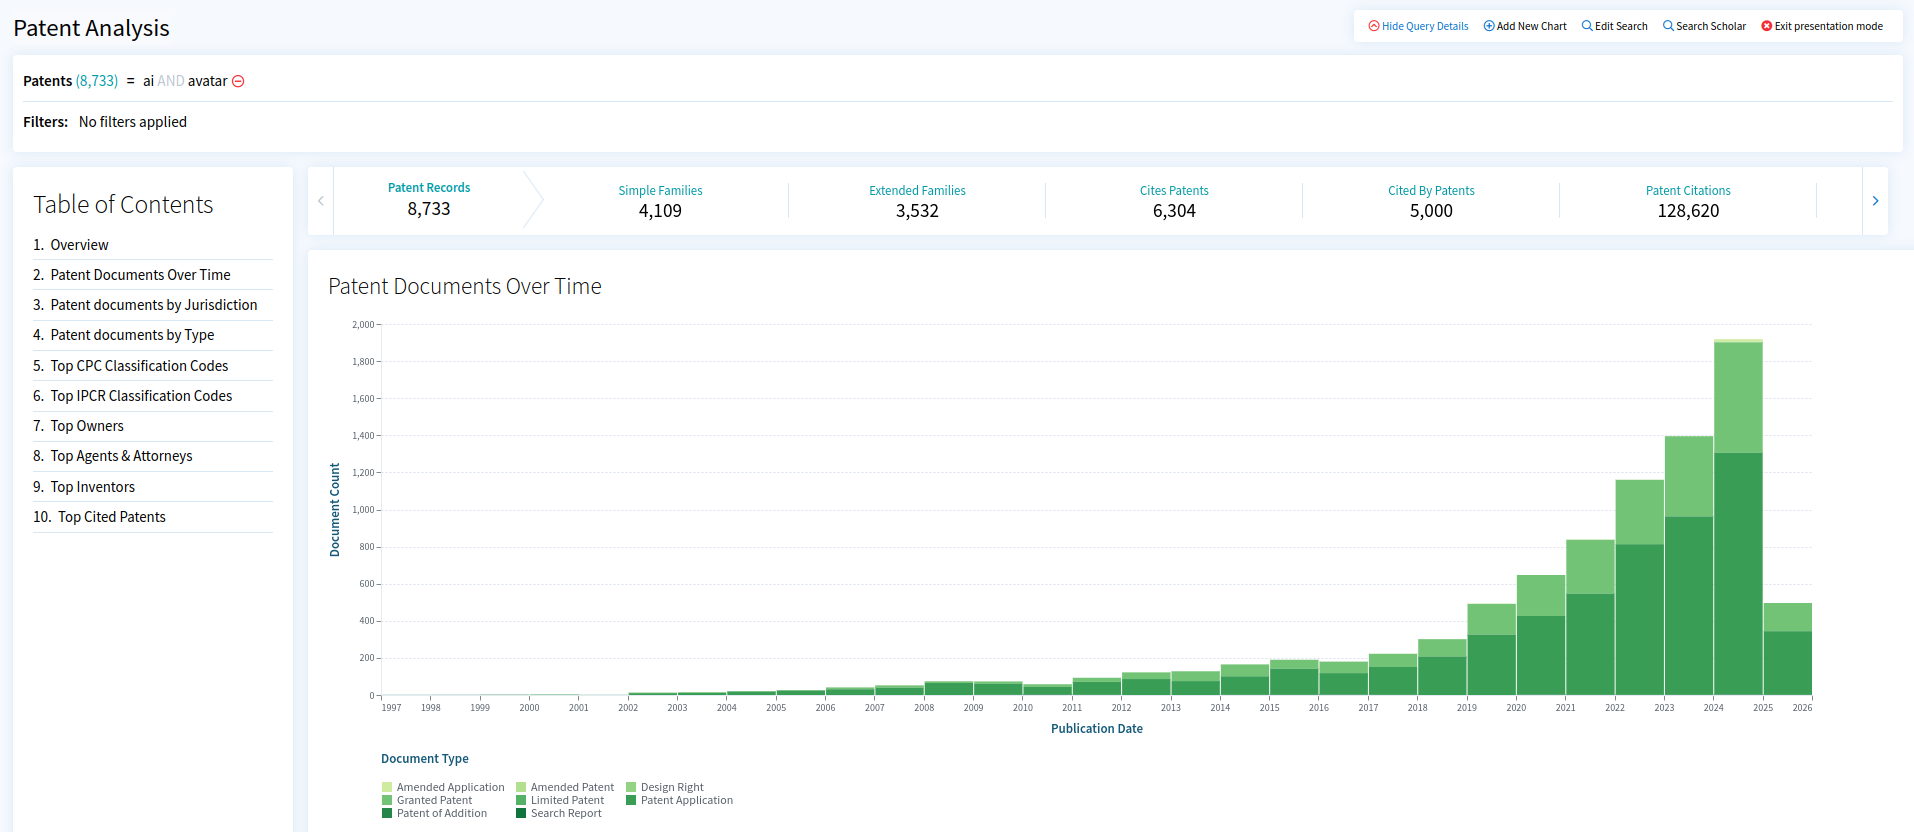
\includegraphics[width=1.0\linewidth]{images/patent-analysis.png}
    \caption{Патентный анализ}
    \label{fig:patent-analysis}
\end{figure}